% !TEX root = ../CourseOT.tex


%%%%%%%%%%%%%%%%%%%%%%%%%%%%%%%%%%%%%%%%%%%%%%%%%%%%%%%%%%%%%%%%%%%%%%%%%%%
%%%%%%%%%%%%%%%%%%%%%%%%%%%%%%%%%%%%%%%%%%%%%%%%%%%%%%%%%%%%%%%%%%%%%%%%%%%
%%%%%%%%%%%%%%%%%%%%%%%%%%%%%%%%%%%%%%%%%%%%%%%%%%%%%%%%%%%%%%%%%%%%%%%%%%%
\section{Wasserstein Estimation}


%%%%%%%%%%%%%%%%%%%%%%%%%%%%%%%%%%%%%%%%%%%%%%%%%%%%%%%%%%%%%%%%%%%%%%%%%
\subsection{Wasserstein Loss}

In statistics, text processing or imaging, one must usually compare a probability distribution $\be$ arising from measurements to a model, namely a parameterized family of distributions $\{\al_\th,\th\in\Theta\}$ where $\Theta$ is a subset of an Euclidean space. Such a comparison is done through a ``loss'' or a ``fidelity'' term, which, in this section, is the Wasserstein distance. 
%
In the simplest scenario, the computation of a suitable parameter $\th$ is obtained by minimizing directly
\eql{\label{eq-wloss-generic}
	\umin{\th \in \Theta} \Ee(\th) \eqdef \MK_\c(\al_\th,\be).
}
Of course, one can consider more complicated problems: for instance, the barycenter problem described in Section~\ref{sec-bary} consists in a sum of such terms. However, most of these more advanced problems can be usually solved by adapting tools defined for basic case: either using the chain rule to compute explicitly derivatives, or using automatic differentiation. %  as advocated in~\S\ref{rem-auto-diff}.

The Wasserstein distance between two histograms or two densities is convex with respect to these inputs, as shown by~\eqref{eq-dual} and~\eqref{eq-dual-generic} respectively. Therefore, when the parameter $\theta$ is itself a histogram, namely $\Theta=\simplex_n$ and $\al_\theta=\theta$, or more generally when $\theta$ describes $K$ weights in the simplex, $\Theta=\simplex_K$, and $\alpha_\theta=\sum_{i=1}^K \theta_i \alpha_i$ is a convex combination of known atoms $\alpha_1,\dots,\alpha_K$ in $\simplex_N$, Problem~\eqref{eq-wloss-generic} remains convex (the first case corresponds to the barycenter problem, the second to one iteration of the dictionary learning problem with a Wasserstein loss~\cite{pmlr-v51-rolet16}). However, for more general parameterizations $\th\mapsto \al_\th$, Problem~\eqref{eq-wloss-generic} is in general not convex. 


A practical problem of paramount importance in statistic and machine learning is density fitting. 
%
Given some discrete samples $(x_i)_{i=1}^n \subset \Xx$ from some unknown distribution, the goal is to fit a parametric model $\th \mapsto \al_\th \in \Mm(\Xx)$ to the observed empirical input measure $\be$
\eql{\label{eq-density-fitting}
	\umin{\th \in \Theta} \Ll(\al_\th,\be)
	\qwhereq
	\be = \frac{1}{n} \sum_i \de_{x_i}, 
}
where $\Ll$ is some ``loss'' function between a discrete and a ``continuous'' (arbitrary) distribution (see Figure~\ref{fig-density-fitting}). 

In the case where $\al_\th$ as a densify $\density{\th} \eqdef \density{\al_\th}$ with respect to the Lebesgue measure (or any other fixed reference measure), the maximum likelihood estimator (MLE) is obtained by solving
\eq{
	\umin{\th} \Ll_{\text{MLE}}(\al_\th,\be) \eqdef -\sum_i \log(\density{\th}(x_i)). 
}
This corresponds to using an empirical counterpart of a Kullback-Leibler loss since, assuming the $x_i$ are i.i.d. samples of some $\bar\be$, then 
\eq{
	\Ll_{\text{MLE}}(\al,\be) \overset{n \rightarrow +\infty}{\longrightarrow} \KL(\al|\bar\be)
}

\begin{figure}
\centering
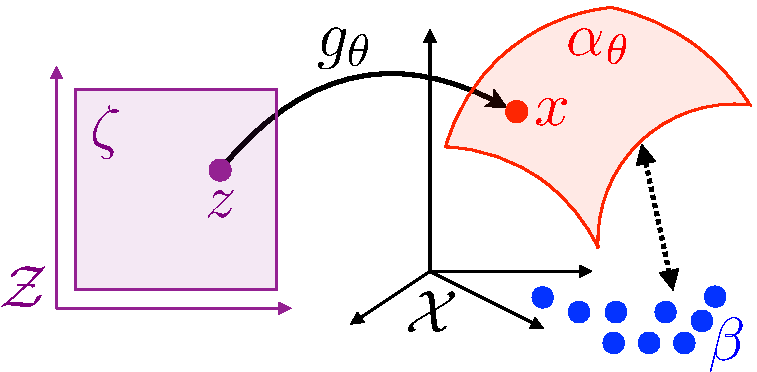
\includegraphics[width=.4\linewidth]{density-fitting/schematic-fitting}
\caption{\label{fig-density-fitting}
Schematic display of the density fitting problem~\ref{eq-density-fitting}.
}
\end{figure}


\newcommand{\fPF}{h}

This MLE approach is known to lead to optimal estimation procedures in many cases (see for instance~\cite{owen2001empirical}). However, it fails to work when estimating singular distributions, typically when the $\al_\th$ does not has a density (so that $\Ll_{\text{MLE}}(\al_\th,\be) = +\infty$) or when $(x_i)_i$ are samples from some singular $\bar\be$ (so that the $\al_\th$ should share the same support as $\be$ for $\KL(\al|\bar\be)$ to be finite, but this support is usually unknown). Another issue is that in several cases of practical interest, the density $\density{\th}$ is inaccessible (or too hard to compute).

A typical setup where both problems (singular and unknown densities) occur is for so-called generative models, where the parametric measure is written as a push-forward of a fixed reference measure $\zeta \in \Mm(\Zz)$
\eq{
	\al_\th = \fPF_{\th,\sharp} \zeta \qwhereq \fPF_\th : \Zz \rightarrow \Xx
}
where the push-forward operator is introduced in Definition~\ref{defn-pushfwd}. The space $\Zz$ is usually low-dimensional, so that the support of $\al_\th$ is localized along a low-dimensional ``manifold'' and the resulting density is highly singular (it does not have a density with respect to Lebesgue measure).
%
Furthermore, computing this density is usually intractable, while generating i.i.d. samples from $\al_\th$ is achieved by computing $x_i=\fPF_\th(z_i)$ where $(z_i)_i$ are i.i.d. samples from $\zeta$.

In order to cope with such difficult scenario, one has to use weak metrics in place of the MLE functional $\Ll_{\text{MLE}}$, which needs to be written in dual form as 
\eql{\label{eq-dual-loss}
	\Ll(\al,\be) \eqdef 
	\umax{(\f,\g) \in \Cc(\X)^2} 
	\enscond{ \int_{\X} \f(x) \d\al(x) + \int_{\X} \g(x) \d\be(x) }{ (\f,\g) \in \Potentials}.
}
Dual norms exposed in Section~\ref{sec-dual-norms} correspond to imposing $\Potentials = \enscond{(\f,-\f)}{\f \in B}$, while optimal transport~\eqref{eq-dual-generic} sets $\Potentials = \Potentials(c)$ as defined in~\eqref{eq-dfn-pot-dual}. 

For a fixed $\th$, evaluating the energy to be minimized in~\eqref{eq-density-fitting} using such a loss function corresponds to solving a semi-discrete optimal transport, which is the focus of Chapter~\ref{c-algo-semidiscr}. Minimizing the energy with respect to $\th$ is much more involved, and is typically highly non-convex.

The class of estimators obtained using $\Ll=\MK_\c$, often called ``Minimum Kantorovitch Estimators'' (MKE), was initially introduced in~\cite{bassetti2006minimum}, see also~\cite{CanasRosasco}.


%%%%%%%%%%%%%%%%%%%%%%%%%%%%%%%%%%%%%%%%%%%%%%%%%%%%%%%%%%%%%%%%%%%%%%%%%
\subsection{Wasserstein Derivatives}

\todo{Write me.}

Eulerian vs Lagrangian. 

Derivatives. 

Sinkhorn smoothing. 



%%%%%%%%%%%%%%%%%%%%%%%%%%%%%%%%%%%%%%%%%%%%%%%%%%%%%%%%%%%%%%%%%%%%%%%%%%%
\subsection{Sample Complexity}

In an applied setting, given two input measures $(\al,\be) \in \Mm_+^1(\X)^2$, an important statistical problem is to approximate the (usually unknown) divergence $D(\al,\be)$ using only samples $(x_i)_{i=1}^n$ from $\al$ and $(y_j)_{j=1}^m$ from $\be$. These samples are assumed to be independently identically distributed from their respective distributions. 
%
For both Wasserstein distances $\Wass_p$ (see~\ref{eq-defn-wass-dist}) and MMD norms (see Section~\ref{sec-dual-norms}), a straightforward estimator of the unknown distance between distributions is compute it directly between the empirical measures, hoping ideally that one can control the rate of convergence of the latter to the former,
\eq{
	D(\al,\be) \approx D(\al_n,\be_m) \qwhereq
	\choice{
		\al_n \eqdef \frac{1}{n}\sum_i \de_{x_i},\\ 
		\be_m \eqdef \frac{1}{m}\sum_j \de_{y_j}.
	}
}
Note that here both $\al_n$ and $\be_m$ are random measures, so $D(\al_n,\be_m)$ is a random number. 
% 
For simplicity, we assume that $\X$ is compact (handling unbounded domain requires extra constraints on the moments of the input measures).

For such a dual distance that metrizes the weak convergence (see Definition~\ref{dfn-weak-conv}), since there is the weak convergence $\hat\al_n \rightarrow \al$, one has $D(\al_n,\be_n) \rightarrow D(\al,\be)$ as $n \rightarrow +\infty$.
%
But an important question is the speed of convergence of $D(\al_n,\be_n)$ toward $D(\al,\be)$, and this rate is often called the ``sample complexity'' of $D$. 

% Note that for $D(\al,\be) = \norm{\cdot}_{\TV}$, since the TV norm does not metrize the weak convergence, $\norm{\al_n - \be_n}_{\TV}$ is not a consistent estimator, namely it does not converge toward $\norm{\al-\be}_{\TV}$. Indeed, with probability 1, $\norm{\al_n - \be_n}_{\TV}=2$ since the support of the two discrete measures does not overlap. Similar issues arise with other $\phi$-divergences, which cannot be estimated using divergences between empirical distributions.

%%%%
\paragraph{Rates for OT.}

For $\X=\RR^\dim$ and measure supported on bounded domain, it is shown by~\cite{dudley1969speed} that for $\dim>2$, and $1 \leq p < +\infty$,  
\eq{
	\EE( |\Wass_p(\al_n,\be_n)-\Wass_p(\al,\be)| ) = O(n^{-\frac{1}{\dim}}),
}
where the expectation $\EE$ is taken with respect to the random samples $(x_i,y_i)_i$. This rate is tight in $\RR^\dim$ if one of the two measures has a density with respect to the Lebesgue measure. This result was proved for general metric spaces~\cite{dudley1969speed} using the notion of covering numbers and was later refined, in particular for $\X=\RR^d$ in~\cite{dereich2013constructive,fournier2015rate}. 
% Proof on $\Wass_1$ implies on $\Wass_p$ for $1 \leq p < +\infty$ by monotonicity in $p$.
This rate can be refined when the measures are supported on low-dimensional subdomains:~\cite{weed2017sharp} show that, indeed, the rate depends on the intrinsic dimensionality of the support. \cite{weed2017sharp} also study the nonasymptotic behavior of that convergence, such as for measures which are discretely approximated (\emph{e.g.} mixture of Gaussians with small variances).
%
It is also possible to prove concentration of $\Wass_p(\al_n,\be_n)$ around its mean $\Wass_p(\al,\be)$; see~\cite{bolley2007quantitative,boissard2011simple,weed2017sharp}.

%%%
\paragraph{Rates for MMD.}

For weak norms $\norm{\cdot}^2_{\Krkhs}$ which are dual of RKHS norms (also called MMD), as defined in~\eqref{eq-kernel-dual}, and contrary to Wasserstein distances, the sample complexity rate does not depend on the ambient dimension 
\eq{
	\EE( |\norm{\al_n-\be_n}_{\Krkhs}^2 - \norm{\al-\be}_{\Krkhs}^2 |^2 )
	= 
	O(n^{-\frac{1}{2}}), 
}
see~\cite{sriperumbudur2012empirical}. Note however that the constant appearing in this rate might depend on the dimension. 
%
This corresponds to the classical rate when using a Monte-Carlo method to estimate an integral using random samples. 
% 
For instance, one has, denoting $\xi=\al-\be$ and $\xi_n=\al_n-\be_n$
\eq{
	\EE( |\norm{\xi_n}_{\Krkhs} - \norm{\al-\be}_{\Krkhs} | ) 	= 
	\EE( |\int k \d(\xi \otimes \xi - \xi_n \otimes \xi_n)|^2 ).
}

\todo{Explain that this corresponds to the Monte-Carlo approximation of integrals using sums. Explain that the constant might depends on the dimension. Give a proof. }

%
% Figure~\ref{fig-sample-complexity} shows a numerical comparison of the sample complexity rates for Wasserstein and MMD distances.  
%
%Note, however, that $\norm{\al_n-\be_n}_{\Krkhs}^2$ is a slightly biased estimate of $\norm{\al-\be}_{\Krkhs}^2$. In order to define an unbiased estimator, and thus to be able to use, for instance, SGD when minimizing such losses, one should rather use the unbiased estimator 
%\begin{align*}
%	\text{MMD}_{\Krkhs}(\al_n,\be_n)^2 & \eqdef
%		\frac{1}{n(n-1)} \sum_{i,i'} \Krkhs(x_i,x_{i'})	+
%		\frac{1}{n(n-1)}\sum_{j,j'} \Krkhs(y_j,y_{j'}) \\
%		 & \qquad - 2
%		\frac{1}{n^2}\sum_{i,j} \Krkhs(x_i,y_j), 
%\end{align*}
%which should be compared to~\eqref{eq-mmd-discr}. It satisfies $\EE(\text{MMD}_{\Krkhs}(\al_n,\be_n)^2) = \norm{\al-\be}_{\Krkhs}^2$; see~\cite{gretton2012kernel}.



%%%
\paragraph{Rates for Sinkhorn.}

\todo{Give the intuition : smoothness of the potentials, Sobolev ball. }


